% STATUS: ACTIVE | COMPARISON READING COPY (2026-09-14) of the versions of the estimated-b filter produced by the
%   substitution e_a = -a' e_dw3 + ((1-a)/b) e_b. Equations only, 0907 conventions; the numbers live in the figures.
%     original      the 0907 core: a_w is a state of its own
%     substituted   the substitution applied to BOTH F_e and the y2 row, a_w kept as a slot (0912)
%     4-state       the self-consistent form: no a_w slot, the gain is computed from the law (0914)
%   A fourth arm exists in code (amodel_fe alone: the substitution in F_e only) but it uses two definitions of the same
%   symbol and is not listed here; it served only to separate the F_e half from the H half of the effect.
%   Sources: 0907_estb_5state_core.tex, 0912_estb_orange_variant.tex, 0914_estb_4state_core.tex.
%   Figures (scripts in test_script/scratch): plot_obs5_variants.m -> figures/obs5_ratio.png, figures/obs5_sigma_V.png
%   (seed 7, 500-step windows, production chord-seed arm); plot_variants_closed_loop.m -> figures/variants_closed_loop.png
%   (plane plant, chord seed, 10 paired seeds).

\documentclass[11pt,a4paper,fontset=none]{ctexart}
\usepackage[fleqn]{amsmath}
\usepackage{amssymb,bm}
\setlength{\mathindent}{0pt}
\usepackage{graphicx}
\usepackage{pdflscape}
\usepackage{geometry}
\geometry{margin=2.0cm}

\setlength{\parindent}{0pt}
\setlength{\parskip}{0.80em}
\linespread{1.08}
\setlength{\abovedisplayskip}{10pt}
\setlength{\belowdisplayskip}{10pt}

\newcommand{\ba}{\bar{a}}
\newcommand{\bw}{\bar{w}}
\newcommand{\ah}{\hat{\ba}_w}
\newcommand{\bh}{\hat{b}}
\newcommand{\wh}{\hat{\bw}}
\newcommand{\ad}{\hat{\ba}_d}
\newcommand{\E}{\mathbb{E}}

\begin{document}

\section{Gain law}

($e_\theta = \theta - \hat\theta$; coefficients at the estimate; $\bw_s$ known)

\begin{align*}
\ba(\bw, b) &= 1 - \frac{1}{b\,(\bw - \bw_s)} \\
\frac{\partial\ba}{\partial\bw} &= b\bigl(1-\ba\bigr)^{2}, \qquad
\frac{\partial^{2}\ba}{\partial\ba\,\partial\bw} = -2\,b\bigl(1-\ba\bigr), \qquad
\Bigl(\frac{\partial\ba}{\partial b}\Bigr)_{\bw,\,\bw_s} = \frac{1-\ba}{b}
\end{align*}

\section{Substitution}

\begin{align*}
e_{\ba_w}[k] &= -\,\bh[k]\bigl(1-\ah[k]\bigr)^{2}e_{\delta\bw_3}[k] + \frac{1-\ah[k]}{\bh[k]}\,e_b[k]
\end{align*}

\section{State}

\begin{align*}
\mathbf{x}^{\text{original}} = \mathbf{x}^{\text{substituted}}
  &= \bigl[\,\delta\bw_1,\ \delta\bw_2,\ \delta\bw_3,\ \ba_w,\ b\,\bigr]^{\top} \\
\mathbf{x}^{\text{4-state}} &= \bigl[\,\delta\bw_1,\ \delta\bw_2,\ \delta\bw_3,\ b\,\bigr]^{\top} \\
\wh[k] &= \bw_d[k] - \delta\hat{\bw}_3[k], \qquad
\ah[k] = 1 - \frac{1}{\bh[k]\bigl(\wh[k] - \bw_s\bigr)}
\end{align*}

\begin{landscape}
\thispagestyle{empty}
\section{Error dynamics}

\subsection*{Original}

\begin{align*}
F_e[k] = {\small\begin{bmatrix}
0 & 1 & 0 & 0 & 0 \\[2pt]
0 & 0 & 1 & 0 & 0 \\[2pt]
0 & 0 & \lambda_c & -F_{dw} & 0 \\[2pt]
0 & 0 & (1-\lambda_c)\,\bh\bigl(1-\ah\bigr)^{2} &
  \begin{array}{l} 1 + \bh\bigl(1-\ah\bigr)^{2}F_{dw} \\[2pt] \quad - 2\bh\bigl(1-\ah\bigr)\bigl(\Delta\bw_d + (1-\lambda_c)\,\delta\hat{\bw}_3\bigr) \end{array} &
  \begin{array}{l} \bigl(1-\ah\bigr)^{2} \\[2pt] \quad \times\bigl(\Delta\bw_d + (1-\lambda_c)\,\delta\hat{\bw}_3\bigr) \end{array} \\[14pt]
0 & 0 & 0 & 0 & 1
\end{bmatrix}}
\end{align*}

\subsection*{Substituted}

\begin{align*}
F_e[k] = {\small\begin{bmatrix}
0 & 1 & 0 & 0 & 0 \\[2pt]
0 & 0 & 1 & 0 & 0 \\[2pt]
0 & 0 & \lambda_c + F_{dw}\,\bh\bigl(1-\ah\bigr)^{2} & 0 & -F_{dw}\dfrac{1-\ah}{\bh} \\[8pt]
0 & 0 &
  \begin{array}{l} (1-\lambda_c)\,\bh\bigl(1-\ah\bigr)^{2} \\[2pt] \quad - F_{dw}\,\bh^{2}\bigl(1-\ah\bigr)^{4} \end{array} &
  1 - 2\bh\bigl(1-\ah\bigr)\bigl(\Delta\bw_d + (1-\lambda_c)\,\delta\hat{\bw}_3\bigr) &
  \begin{array}{l} \bigl(1-\ah\bigr)^{2}\bigl(\Delta\bw_d + (1-\lambda_c)\,\delta\hat{\bw}_3\bigr) \\[2pt] \quad + F_{dw}\bigl(1-\ah\bigr)^{3} \end{array} \\[14pt]
0 & 0 & 0 & 0 & 1
\end{bmatrix}}
\end{align*}

\subsection*{4-state}

\begin{align*}
F_e[k] = {\small\begin{bmatrix}
0 & 1 & 0 & 0 \\[2pt]
0 & 0 & 1 & 0 \\[2pt]
0 & 0 & \lambda_c + F_{dw}\,\bh\bigl(1-\ah\bigr)^{2} & -F_{dw}\dfrac{1-\ah}{\bh} \\[8pt]
0 & 0 & 0 & 1
\end{bmatrix}}
\end{align*}
\end{landscape}

\section{Measurement}

$\bigl(\nabla_d\bw_d[k] = \bw_d[k] - \bw_d[k-d]$;\ \
$\ad[k] = 1 - 1/\bigl[\bh[k]\bigl(\wh[k] - \nabla_d\bw_d[k] - \bw_s\bigr)\bigr]\bigr)$

\subsection*{Original}

\begin{align*}
H[k] = \begin{bmatrix}
1 & 0 & 0 & 0 & 0 \\[2pt]
0 & 0 & 0 & 1 + 2\bh\bigl(1-\ah\bigr)\nabla_d\bw_d & -\bigl(1-\ah\bigr)^{2}\nabla_d\bw_d
\end{bmatrix}
\end{align*}

\subsection*{Substituted}

\begin{align*}
H[k] = \begin{bmatrix}
1 & 0 & 0 & 0 & 0 \\[6pt]
0 & 0 &
  \begin{array}{l} -\Bigl(1 + 2\bh\bigl(1-\ah\bigr)\nabla_d\bw_d\Bigr) \\[2pt] \quad \times\bh\bigl(1-\ah\bigr)^{2} \end{array} & 0 &
  \begin{array}{l} \Bigl(1 + 2\bh\bigl(1-\ah\bigr)\nabla_d\bw_d\Bigr)\dfrac{1-\ah}{\bh} \\[4pt] \quad - \bigl(1-\ah\bigr)^{2}\nabla_d\bw_d \end{array}
\end{bmatrix}
\end{align*}

\subsection*{4-state}

\begin{align*}
H[k] = \begin{bmatrix}
1 & 0 & 0 & 0 \\[2pt]
0 & 0 & -\bh\bigl(1-\ad\bigr)^{2} & \dfrac{1-\ad}{\bh}
\end{bmatrix}
\end{align*}

\clearpage
\section{Observability}

($\mathbf{e}[k]$ the error vector of the version at hand, $n$ its length;
$\mathbf{n}[k] = [\,n_w[k],\ n_a[k]\,]^{\top}$ \\
$\Phi(k,k_0) := F_e[k-1]\,F_e[k-2]\cdots F_e[k_0]$, $\Phi(k_0,k_0) = I$ \\
$N$ window length \\
$\mathbf{Y} := [\,\mathbf{e}_y[k_0];\ \dots;\ \mathbf{e}_y[k_0+N]\,]$,
$\mathbf{N} := [\,\mathbf{n}[k_0];\ \dots;\ \mathbf{n}[k_0+N]\,]$ \\
$X_{:,j}$ column $j$ of $X$)

\begin{align*}
\mathbf{e}[k]   &= \Phi(k,k_0)\,\mathbf{e}[k_0] \\
\mathbf{e}_y[k] &= H[k]\,\Phi(k,k_0)\,\mathbf{e}[k_0] + \mathbf{n}[k] \\
\mathbf{Y}      &= O(k_0,N)\,\mathbf{e}[k_0] + \mathbf{N}, \qquad
O(k_0,N) := \begin{bmatrix} H[k_0]\,\Phi(k_0,k_0) \\ H[k_0+1]\,\Phi(k_0+1,k_0) \\ \vdots \\ H[k_0+N]\,\Phi(k_0+N,k_0) \end{bmatrix}
\end{align*}

\begin{align*}
R_w &:= \mathrm{diag}\bigl(R[k_0],\ \dots,\ R[k_0+N]\bigr), \qquad
O_w(k_0,N) := R_w^{-1/2}\,O(k_0,N) \\
\mathbf{Y}_w &:= R_w^{-1/2}\,\mathbf{Y} = O_w(k_0,N)\,\mathbf{e}[k_0] + \mathbf{N}_w, \qquad
\E\bigl[\mathbf{N}_w\mathbf{N}_w^{\top}\bigr] = I
\end{align*}

\begin{align*}
O_w(k_0,N)\,\mathbf{v}_i &= \sigma_i\,\mathbf{u}_i, \qquad i = 1,\dots,n, \qquad
\|\mathbf{v}_i\| = \|\mathbf{u}_i\| = 1 \\
\sigma_1 &\ge \dots \ge \sigma_n \ge 0 \\
\sigma_1 &= \max_{\|\mathbf{v}\|=1}\|O_w(k_0,N)\,\mathbf{v}\|, \qquad
\sigma_n = \min_{\|\mathbf{v}\|=1}\|O_w(k_0,N)\,\mathbf{v}\| \\
\operatorname{rank} O_w(k_0,N) &= \#\{\,i : \sigma_i > 0\,\} \\
F_e[k]_{:,j} = f_j[k]\,I_{:,j},\ \ H[k]_{:,j} = \mathbf{0}\ \ \forall k
  &\ \Rightarrow\ O_w(k_0,N)_{:,j} = \mathbf{0} \\
  &\ \Rightarrow\ \sigma_n = 0
\end{align*}

\subsection*{The two columns}

\begin{align*}
\text{original:}\quad
F_{e,:,\ba_w} &= \Bigl[\,0,\ 0,\ -F_{dw},\
  1 + \bh\bigl(1-\ah\bigr)^{2}F_{dw} - 2\bh\bigl(1-\ah\bigr)\bigl(\Delta\bw_d + (1-\lambda_c)\,\delta\hat{\bw}_3\bigr),\ 0\,\Bigr]^{\top} \\
H_{:,\ba_w} &= \Bigl[\,0,\ 1 + 2\bh\bigl(1-\ah\bigr)\nabla_d\bw_d\,\Bigr]^{\top} \\[6pt]
\text{substituted:}\quad
F_{e,:,\ba_w} &= \Bigl[1 - 2\bh\bigl(1-\ah\bigr)\bigl(\Delta\bw_d + (1-\lambda_c)\,\delta\hat{\bw}_3\bigr)\Bigr]\,I_{:,\ba_w} \\
H_{:,\ba_w} &= \mathbf{0}
\end{align*}

\begin{align*}
\text{original:}\quad
F_{e,:,b} &= \Bigl[\,0,\ 0,\ 0,\ \bigl(1-\ah\bigr)^{2}\bigl(\Delta\bw_d + (1-\lambda_c)\,\delta\hat{\bw}_3\bigr),\ 1\,\Bigr]^{\top}, &
H_{:,b} &= \Bigl[\,0,\ -\bigl(1-\ah\bigr)^{2}\nabla_d\bw_d\,\Bigr]^{\top} \\[6pt]
\text{4-state:}\quad
F_{e,:,b} &= \Bigl[\,0,\ 0,\ -F_{dw}\dfrac{1-\ah}{\bh},\ 1\,\Bigr]^{\top}, &
H_{:,b} &= \Bigl[\,0,\ \dfrac{1-\ad}{\bh}\,\Bigr]^{\top}
\end{align*}

\begin{align*}
\Delta\bw_d[k] = 0\ \ \forall k \quad&\Longrightarrow\quad F_{dw} \to 0, \qquad \nabla_d\bw_d = 0 \\
&\Longrightarrow\quad H^{\text{original}}_{:,b} = \mathbf{0}, \qquad
H^{\text{4-state}}_{:,b} = \Bigl[\,0,\ \frac{1-\ah}{\bh}\,\Bigr]^{\top} \neq \mathbf{0}
\end{align*}

\subsection*{Ratios}

\begin{align*}
\frac{\sigma_5}{\sigma_1}\ \ (n = 5), \qquad \frac{\sigma_4}{\sigma_1}\ \ (n = 4), \qquad
\frac{\sigma_n}{\sigma_1} = 0 \iff \exists\,j:\ O_w(k_0,N)_{:,j} = \mathbf{0}
\end{align*}

\clearpage
\thispagestyle{empty}
\noindent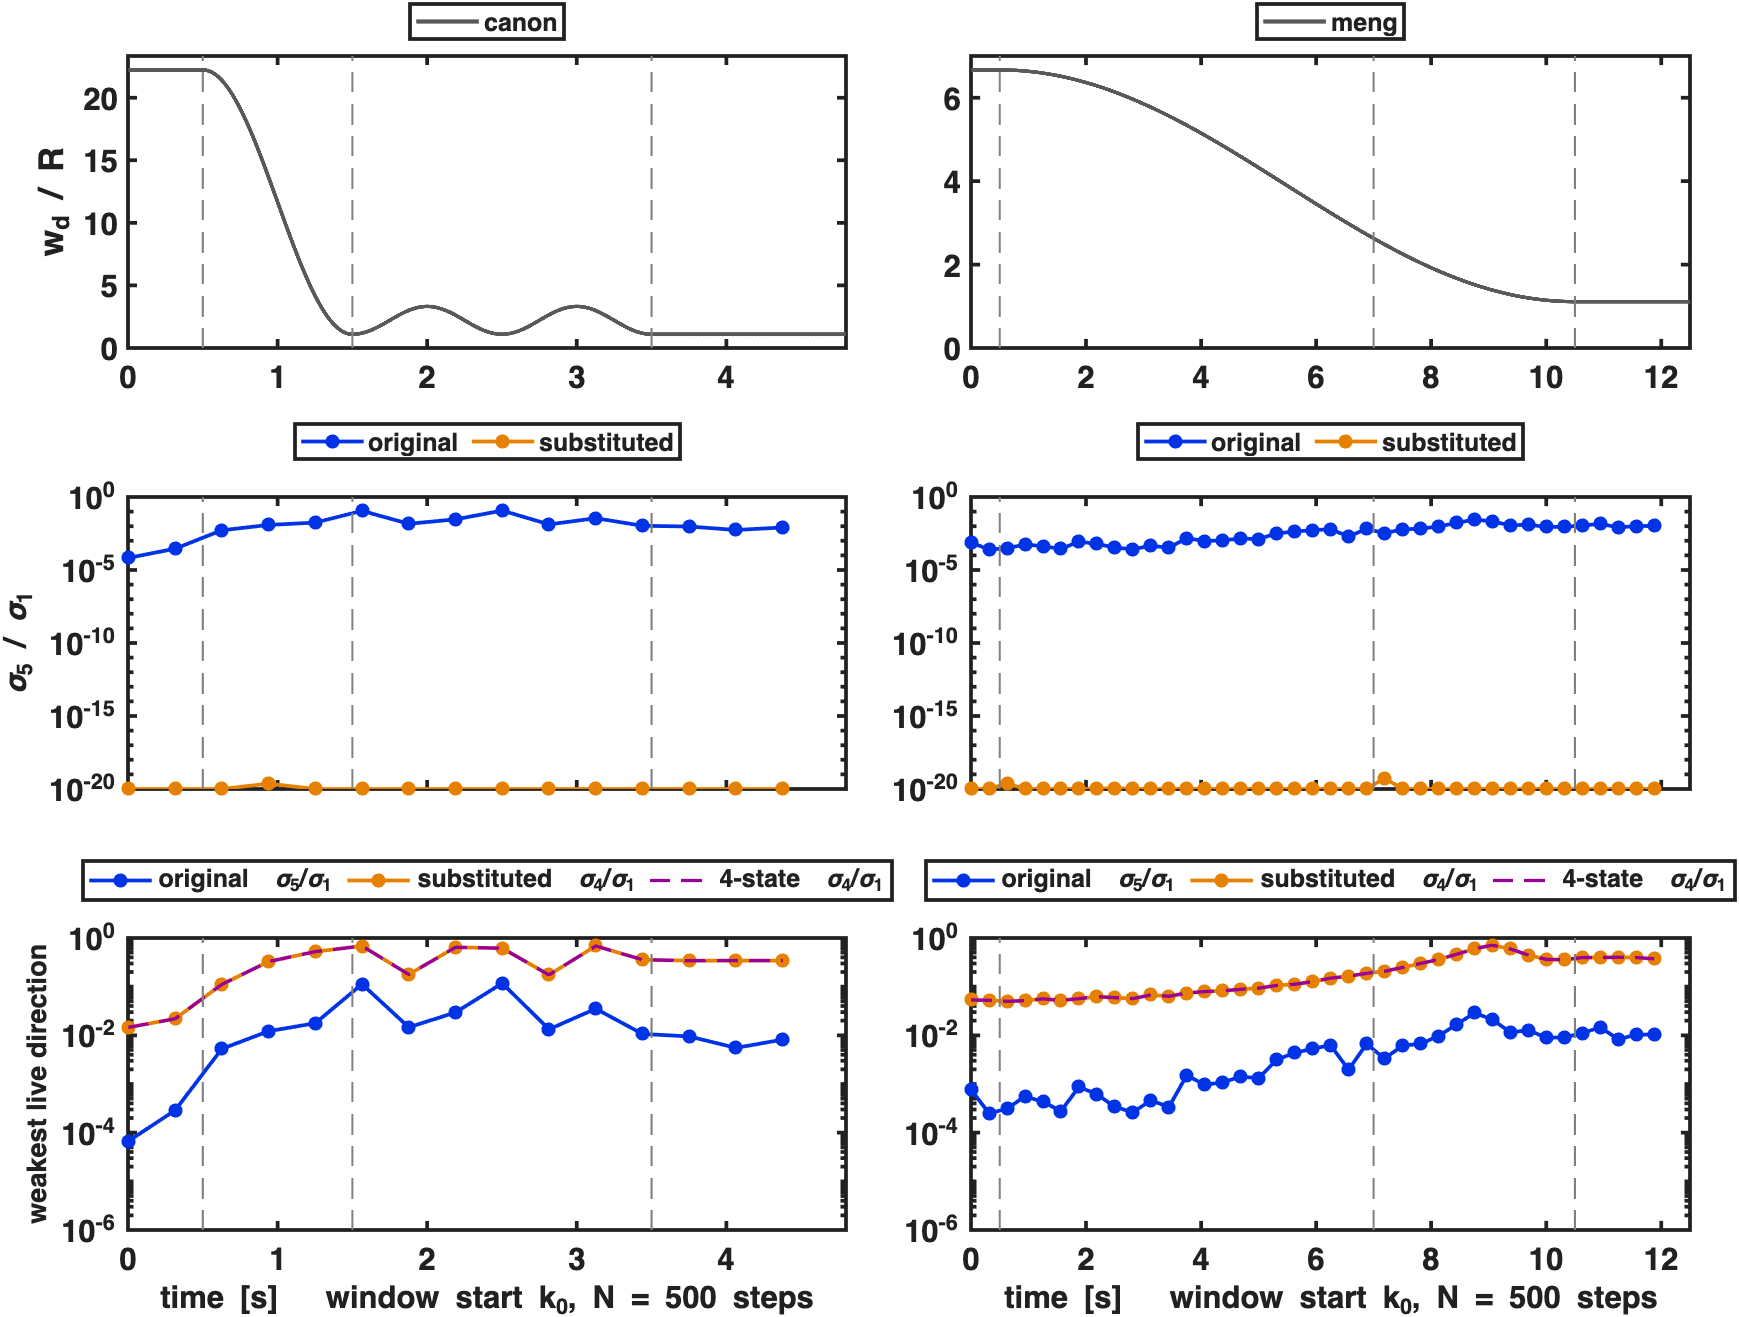
\includegraphics[width=\textwidth]{figures/obs5_ratio.png}

\clearpage
\thispagestyle{empty}
\noindent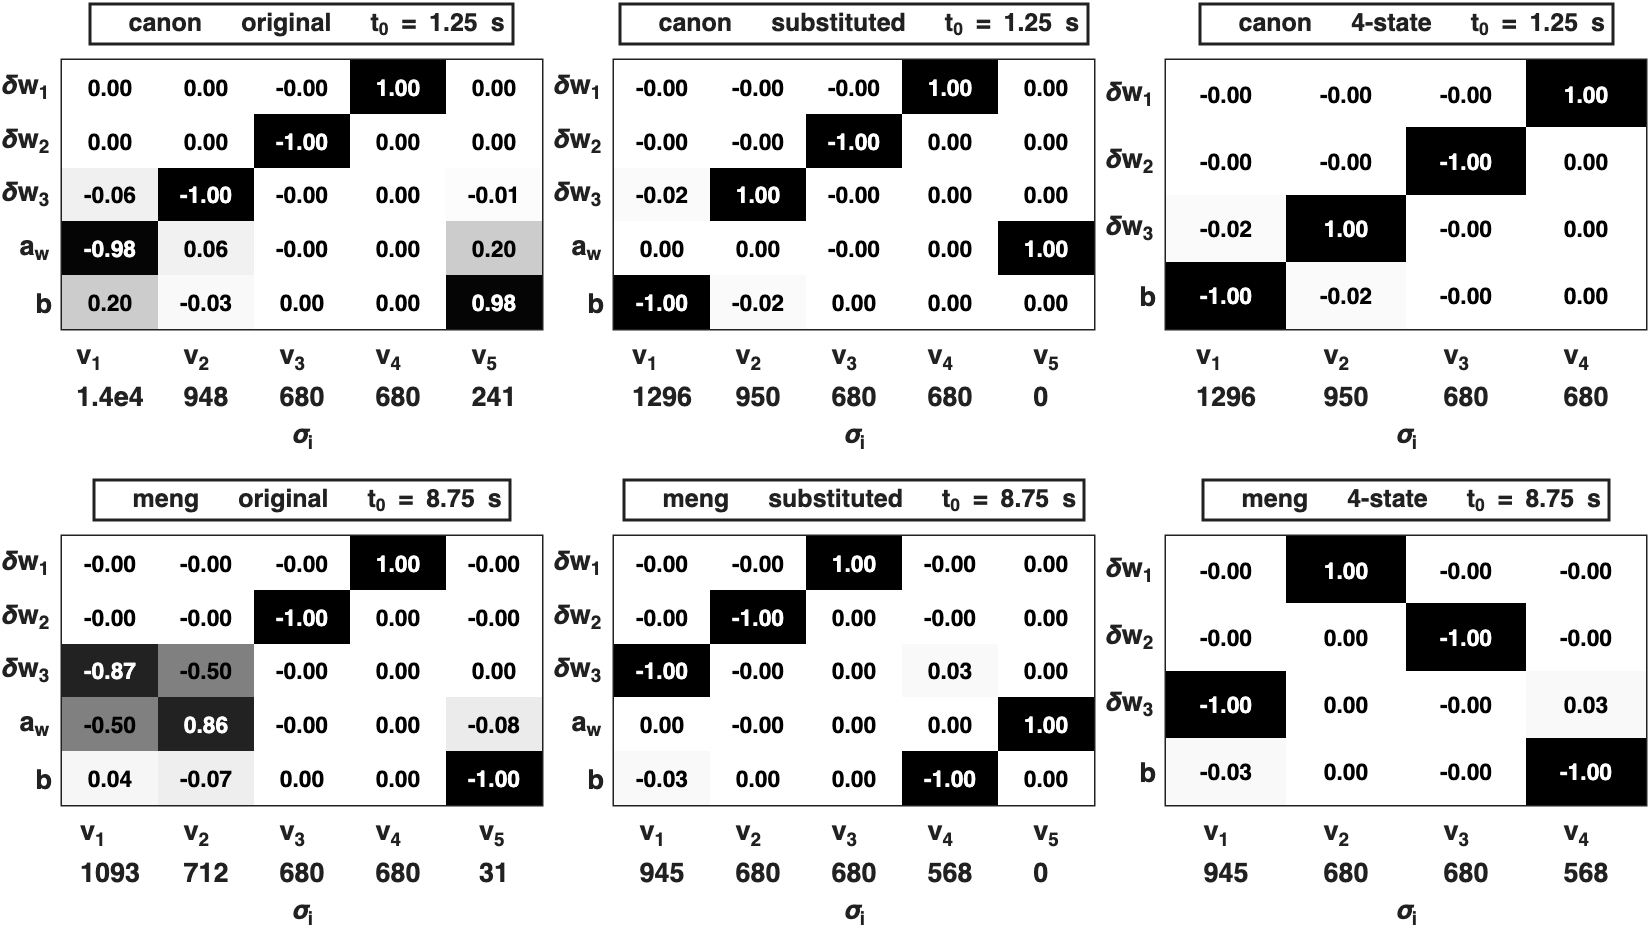
\includegraphics[width=\textwidth]{figures/obs5_sigma_V.png}

\clearpage
\thispagestyle{empty}
\noindent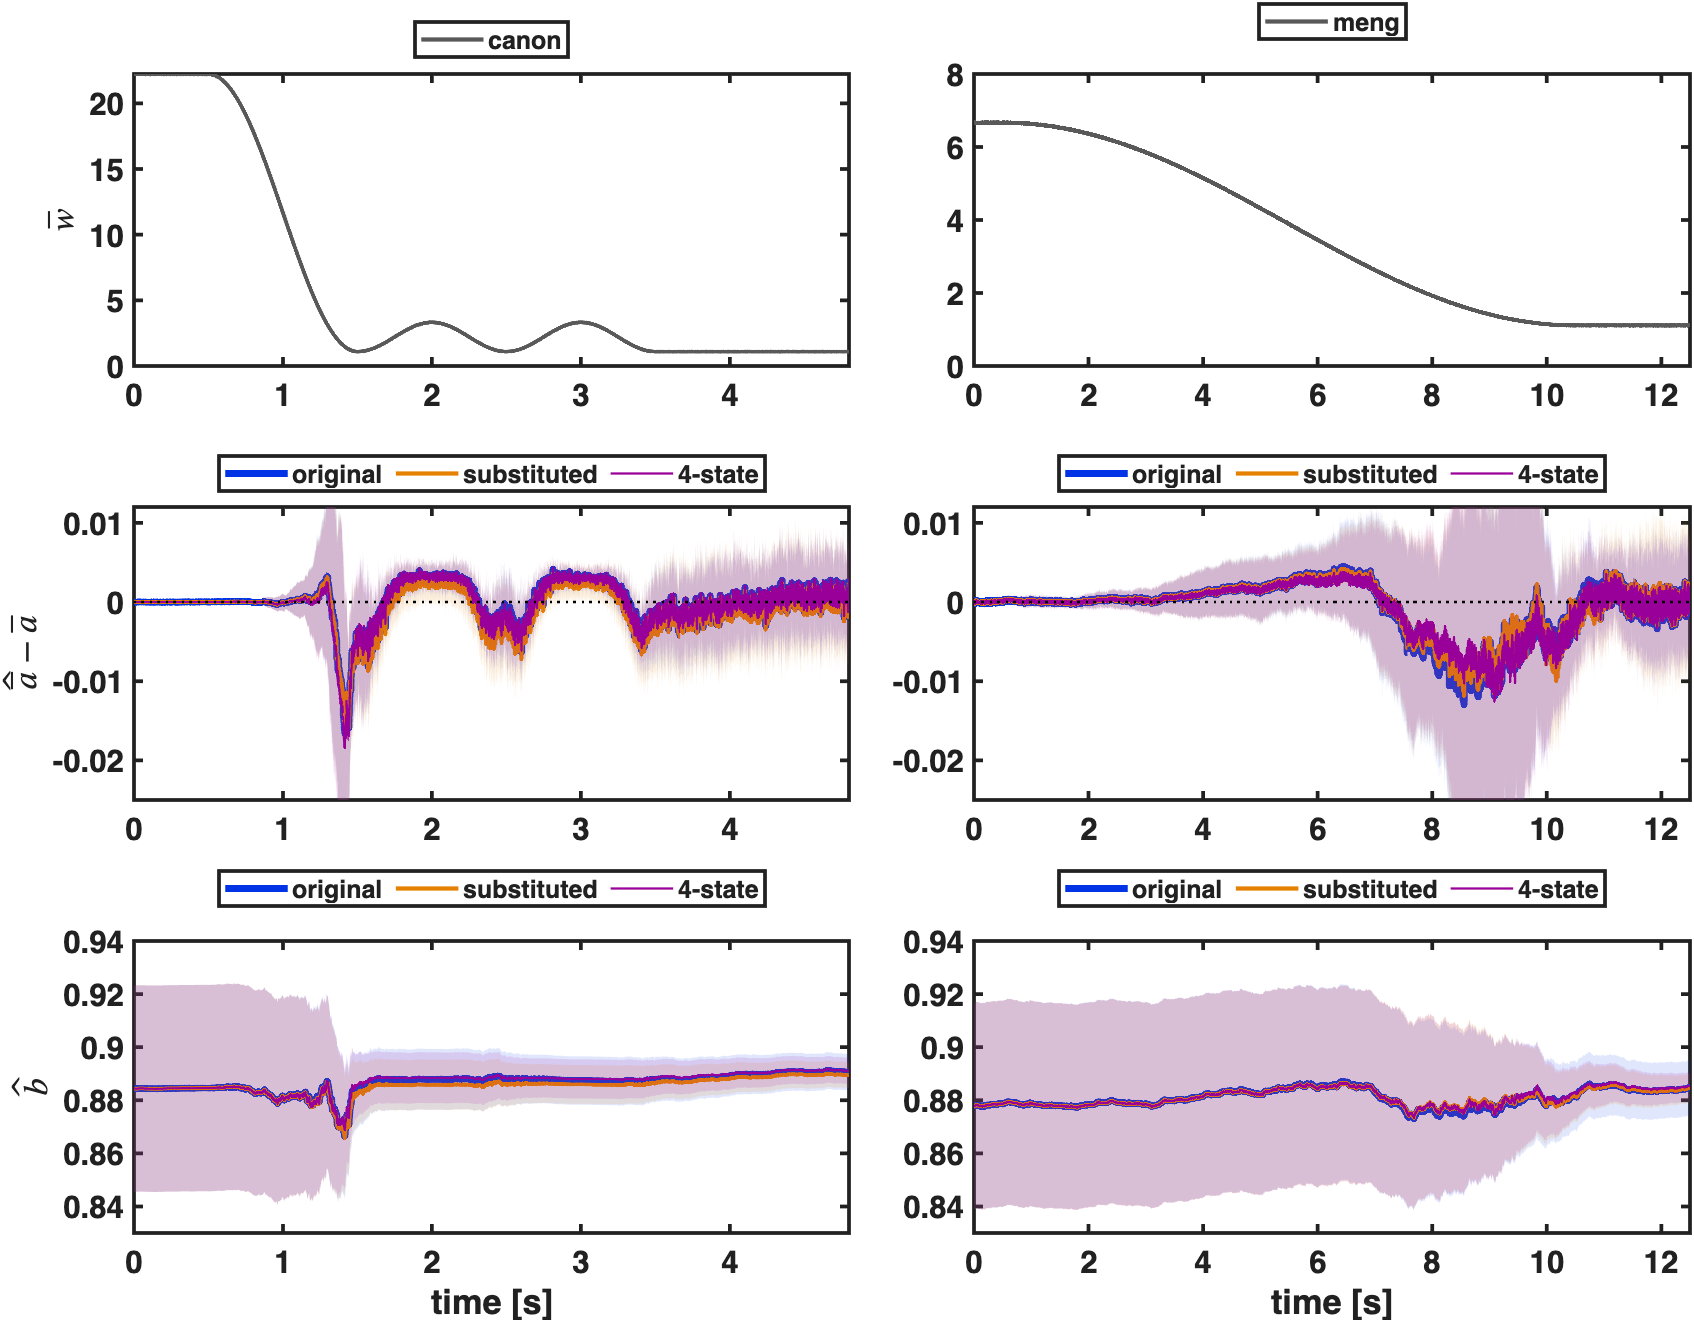
\includegraphics[width=\textwidth]{figures/variants_closed_loop.png}

\end{document}
